\documentclass[11pt,a4paper]{article}
\usepackage[T1]{fontenc}
\usepackage[utf8]{inputenc}
\usepackage[american]{babel}
\usepackage{textcomp}
\usepackage{graphicx}
\usepackage{booktabs}
\usepackage{array}
\usepackage{longtable}
\usepackage{float}
\usepackage{fancyvrb}
\usepackage{ragged2e}
\usepackage[nochapters,beramono,eulermath,pdfspacing,dottedtoc]{classicthesis}

% type area (matches the DSS classicthesis template and the literature review)
\areaset[current]{360pt}{632pt}
\setlength{\footskip}{21pt}
\addtolength{\voffset}{48.4pt}
\setlength{\marginparwidth}{7em}
\setlength{\marginparsep}{2em}

\newcommand{\myTitle}{Cross-Dataset Generalisation of Deep Learning for Malaria Classification in Microscopy Images}
\newcommand{\myName}{Noah Tjon Sien Kie}
\newcommand{\myStudentNumber}{2103939}
\newcommand{\myCommittee}{Dr.\ Sharon Ong}
\newcommand{\myDate}{11 November 2026}
\newcommand{\myStage}{Deliverable D4, Capstone Portfolio}
\newcommand{\repourl}{https://gitlab.uvt.nl/capstone/2026-fall/u927271}

\usepackage{scrextend}
\newlength{\titlelogoskip}\setlength{\titlelogoskip}{-49.6pt}
\newlength{\titlegapA}\setlength{\titlegapA}{141.8pt}
\newlength{\titlegapB}\setlength{\titlegapB}{65pt}
\newlength{\titlegapC}\setlength{\titlegapC}{33pt}
\newlength{\bodytitleskip}\setlength{\bodytitleskip}{23.1pt}
\newlength{\bodygapA}\setlength{\bodygapA}{31.4pt}
\newlength{\bodygapB}\setlength{\bodygapB}{13.6pt}
\newlength{\backindent}\setlength{\backindent}{24pt}
\newlength{\backtopskip}\setlength{\backtopskip}{-15.7pt}

\definecolor{ctcite}{rgb}{0.05,0.05,0.50}
\hypersetup{colorlinks=true, linkcolor=ctcite, citecolor=ctcite, urlcolor=ctcite,
  pdftitle={\myTitle: Technical Report}, pdfauthor={\myName}, breaklinks=true}

\usepackage[style=apa,backend=biber,natbib=true]{biblatex}
\DeclareLanguageMapping{american}{american-apa}
\addbibresource{refs.bib}
\defbibheading{ctbib}[References]{%
  \section*{\spacedlowsmallcaps{#1}}%
  \markright{\spacedlowsmallcaps{#1}}}

\setlength{\LTcapwidth}{\linewidth}
\setlength{\emergencystretch}{3em}
\setlength{\LTpre}{6pt}
\setlength{\LTpost}{6pt}

\begin{document}
\frenchspacing
\raggedbottom
\pagestyle{empty}

\begin{titlepage}
  \begin{center}
    \vspace*{\titlelogoskip}
    
\includegraphics[width=167pt]{tilburg-logo}
    \vspace{\titlegapA}

    {\huge\rmfamily\normalfont\spacedallcaps{\myTitle}\par}
    \vspace{\titlegapB}
    {\normalsize\spacedlowsmallcaps{\myName}\par}
    \vspace{\titlegapC}
    {\footnotesize\spacedlowsmallcaps{Technical Report}\par}
    \vspace{4pt}
    {\footnotesize\spacedlowsmallcaps{Capstone Project, MSc Data Science \& Society, Tilburg University}\par}
    \vfill
  \end{center}
\end{titlepage}

\thispagestyle{empty}
\begin{addmargin}[\backindent]{0pt}
\noindent
\vspace*{\backtopskip}

\noindent\spacedlowsmallcaps{Student Number}

\vspace{7.5pt}\noindent\myStudentNumber

\vspace{15.1pt}

\noindent\spacedlowsmallcaps{Supervisor}

\vspace{7.5pt}\noindent\myCommittee

\vspace{15.1pt}

\noindent\spacedlowsmallcaps{Panel}

\vspace{7.5pt}\noindent to be confirmed

\vspace{15.1pt}

\noindent\spacedlowsmallcaps{Course}

\vspace{7.5pt}\noindent Capstone Project, MSc Data Science \& Society, Tilburg University

\vspace{15.1pt}

\noindent\spacedlowsmallcaps{Location}

\vspace{7.5pt}\noindent Tilburg University\\
School of Humanities and Digital Sciences\\
Department of Cognitive Science \&\\
Artificial Intelligence\\
Tilburg, The Netherlands

\vspace{15.1pt}

\noindent\spacedlowsmallcaps{Date}

\vspace{7.5pt}\noindent\myDate\ (\myStage)

\vspace{15.1pt}

\noindent\spacedlowsmallcaps{Word count}

\vspace{7.5pt}\noindent 2,750

\vspace{15.1pt}

\noindent\spacedlowsmallcaps{Repository}

\vspace{7.5pt}\noindent\url{\repourl}
\end{addmargin}

\clearpage
\pagestyle{scrheadings}
\rofoot[{\small\thepage}]{}
\setcounter{page}{1}
\thispagestyle{plain}

\begin{center}
  \vspace*{\bodytitleskip}
  {\LARGE\rmfamily\normalfont\spacedallcaps{Technical Report}\par}
  \vspace{\bodygapA}
  {\normalsize\spacedlowsmallcaps{\myName}\par}
  \vspace{\bodygapB}
\end{center}

\section*{Abstract}

Convolutional neural networks (CNNs) that classify red blood cells as malaria-infected score almost perfectly on the public NIH dataset but worse on images from other laboratories. This project measures that drop and tests two suspected causes: crop format and stain colour. ImageNet-pretrained VGG-16, ResNet-50 and \mbox{MobileNetV2} were fine-tuned on NIH cells and tested unchanged on the external datasets BBBC041 and MP-IDB. Sensitivity fell by up to 63 percentage points, and the smallest network lost the most. Removing the background or matching stain colour at test time did not, on average, improve how well the models rank infected above uninfected cells (AUC). These two differences therefore do not explain the drop.

\section{Introduction}

Malaria caused an estimated 282 million cases and 610,000 deaths in 2024 \citep{who2025}. Diagnosis still relies on a trained microscopist reading a stained blood smear \citep{rajaraman2018}, and many remote areas have limited access to good-quality microscopy \citep{whordt}. Automated cell classification could help, if it stays accurate across laboratories.

The task is binary classification of single red-blood-cell images as parasitised or uninfected. Pretrained convolutional neural networks (CNNs) are trained on the NIH dataset and tested on two external datasets, BBBC041 and MP-IDB. The drop is the loss in sensitivity or specificity relative to held-out NIH patients. Stakeholders are analysed in the \href{https://gitlab.uvt.nl/capstone/2026-fall/u927271/-/blob/main/docs/elsa_report.md}{ELSA report}.

\textbf{MRQ.} To what extent do pretrained CNNs trained to classify NIH single-cell images as parasitised or uninfected lose sensitivity on BBBC041 and MP-IDB, and specificity on BBBC041, relative to a patient-grouped NIH hold-out set, and which dataset differences explain this drop?

\textbf{RQ1.} How large is the drop from the patient-grouped NIH hold-out set, in percentage points, for \mbox{MobileNetV2}, ResNet-50 and VGG-16 applied without fine-tuning to BBBC041 and MP-IDB, and does the lighter architecture lose less than the heavier ones?

\textbf{RQ2.} What share of the RQ1 drop is recovered when test cells are matched to NIH at test time, first in crop format (background removed) and then in stain colour (Reinhard or histogram matching)?

\textbf{RQ3.} Does sensitivity on the pooled different-species MP-IDB cells (\emph{n} = 140) differ from \emph{P. falciparum} (\emph{n} = 1,297) by more than the resampling interval, and which BBBC041 life stages account for the largest share of missed parasites?

Sections 2 to 5 cover the literature, method, results and conclusions.

\section{Literature review}

On NIH itself, \citet{rajaraman2018} reached 98.6\% accuracy when cells were split at random but 95.9\% when patients were kept apart, so random splits inflate the baseline. \citet{zhao2020} tested an NIH-trained VGG-16 on BBBC041, where its AUC fell from 0.994 to 0.945. \citet{loddo2022} found light and heavy CNNs similar within NIH, yet NIH-trained models averaged only 60.61\% when separating rings, the earliest parasite stage, from later stages on MP-IDB. \citet{hou2026}, the state of the art and the protocol adopted here, split NIH by patient and tested on external datasets; their compact model kept 96.4\% sensitivity on BBBC041 but reached only 18.0\% specificity. \citet{xu2025} showed that colour normalisation of malaria smears depends strongly on the method: accuracy at classifying parasite stages across imaging platforms was 29.34\% after Reinhard colour transfer and 48.66\% with BeerLaNet, their learned stain-normalisation network.

Three gaps follow. First, the drop has been reported with different metrics and decision thresholds and for different models, so its size and its dependence on architecture are unclear. Second, crop format (NIH cells cut out onto black, external cells cut as rectangles with background) and stain colour are named as suspected causes \citep{zhao2020,loddo2022,hou2026}, but no study changes one of them while keeping the model fixed. Third, none reports how much of the drop such a change recovers. This project addresses all three: three architectures under one protocol, and test images edited one difference at a time while the models stay fixed.

\section{Methodology}

Figure 1 shows the pipeline; sections of the Methodology Overview (MO) in the repository document each step.

\begin{figure}[H]
\centering
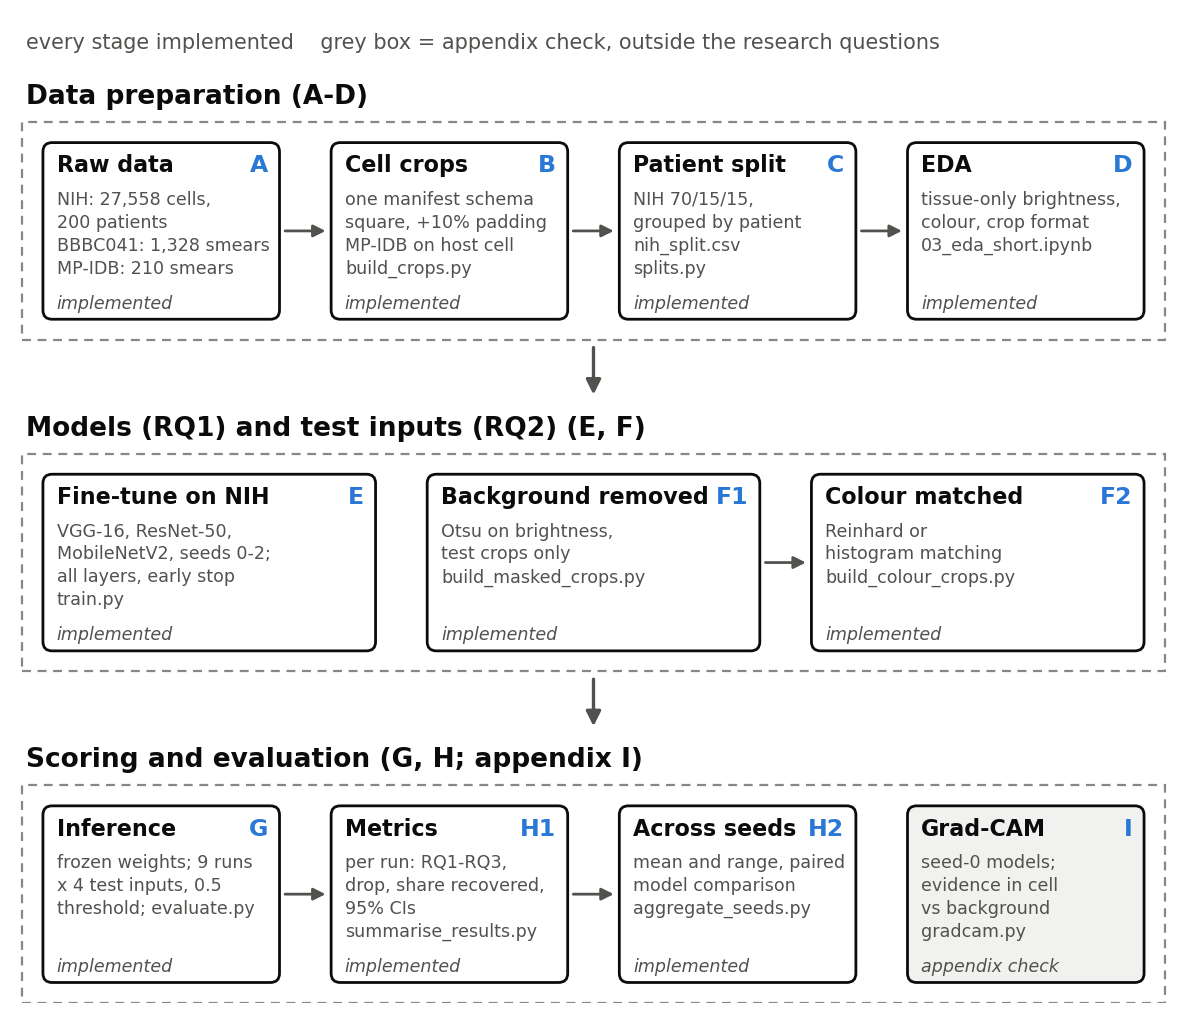
\includegraphics[width=\linewidth,height=0.66\textheight,keepaspectratio]{figures/pipeline_v4.png}
\caption{Pipeline. F1 and F2 are the two RQ2 steps; each box names the script that implements it. Drawn by \texttt{scripts/\allowbreak{}make\_\allowbreak{}mo\_\allowbreak{}figures.\allowbreak{}py}.}
\end{figure}

\subsection{Data}

The training data are the NIH cell images, from the US National Library of Medicine \citep{rajaraman2018}: 27,558 red blood cells from 200 patients in Chittagong, Bangladesh, half infected with the parasite \emph{Plasmodium falciparum}, each cut out along its outline and placed on a black square. They were split 70/15/15 by patient, so no model is tested on a patient it was trained on; the 30 hold-out patients, never used in training, give the reference performance (MO \S{}3.2).

Two external datasets are used for testing only. BBBC041 \citep{ljosa2012} contains \emph{P. vivax} smears photographed in two batches, kept apart as site\_a (79,569 cells, 2.7\% parasitised) and site\_b (5,917 cells, 5.1\%). Ambiguous cells (446, marked ``difficult'') and white blood cells (103) were excluded. MP-IDB \citep{loddo2019} marks only parasites, so it has no uninfected cells. Each of its 1,437 parasites was cropped around the red cell containing it, like NIH's whole-cell crops, and grouped into \emph{P. falciparum} (1,297) and three other species (140) (MO \S{}3.1). Exploratory analysis (MO \S{}4) found that a median 26\% of each NIH crop is black frame, whereas test crops show background and neighbouring cells, and that BBBC041 cells carry three to four times more blue stain.

\subsection{Models and training}

Three CNNs pretrained on ImageNet, 1.2 million labelled photographs \citep{russakovsky2015}, were used: \mbox{MobileNetV2} \citep{sandler2018}, ResNet-50 \citep{he2016} and VGG-16 \citep{simonyan2015}, with 2.2, 23.5 and 134.3 million parameters (learned weights). Each network's last layer was replaced by one output, the probability that the cell is parasitised, and all layers were fine-tuned (trained further on NIH), because features learned from everyday photographs do not fit stained cells. All three used the same settings (Appendix Table A4): flips and 90\textdegree{} rotations as augmentation, and early stopping, which ends training when the error on NIH validation patients stops falling and keeps the best model so far. Hyperparameters (training settings) were fixed, not tuned per model, so RQ1 compares architectures rather than tuning budgets. Random colour changes were left out on purpose: they teach a model to ignore colour, and RQ2 could then not show how much colour matters. Training is random, so each architecture was trained three times (seeds 0, 1 and 2; MO \S{}5.1, \S{}5.3).

\subsection{Test-time ablation (RQ2)}

RQ2 edits only the test images, so any change in the fixed models' performance comes from the edit. Step F1 removes the background with Otsu's method \citep{otsu1979}, which picks the brightness threshold that best separates cell from surroundings: everything outside the cell becomes black, as in NIH crops. Its masks matched hand-drawn NIH outlines with a median Dice overlap of 0.90 (1 is perfect), while the neural model U\textsuperscript{2}-Net found no cell in 21\% of NIH crops (MO \S{}5.2). Step F2 then matches stain colour to NIH in two separate variants: Reinhard transfer \citep{reinhard2001} matches the mean and spread of each cell's colour channels to NIH, and histogram matching maps each colour channel's whole distribution onto NIH's (reference: 1,000 NIH training cells; Figure 2).

\begin{figure}[H]
\centering
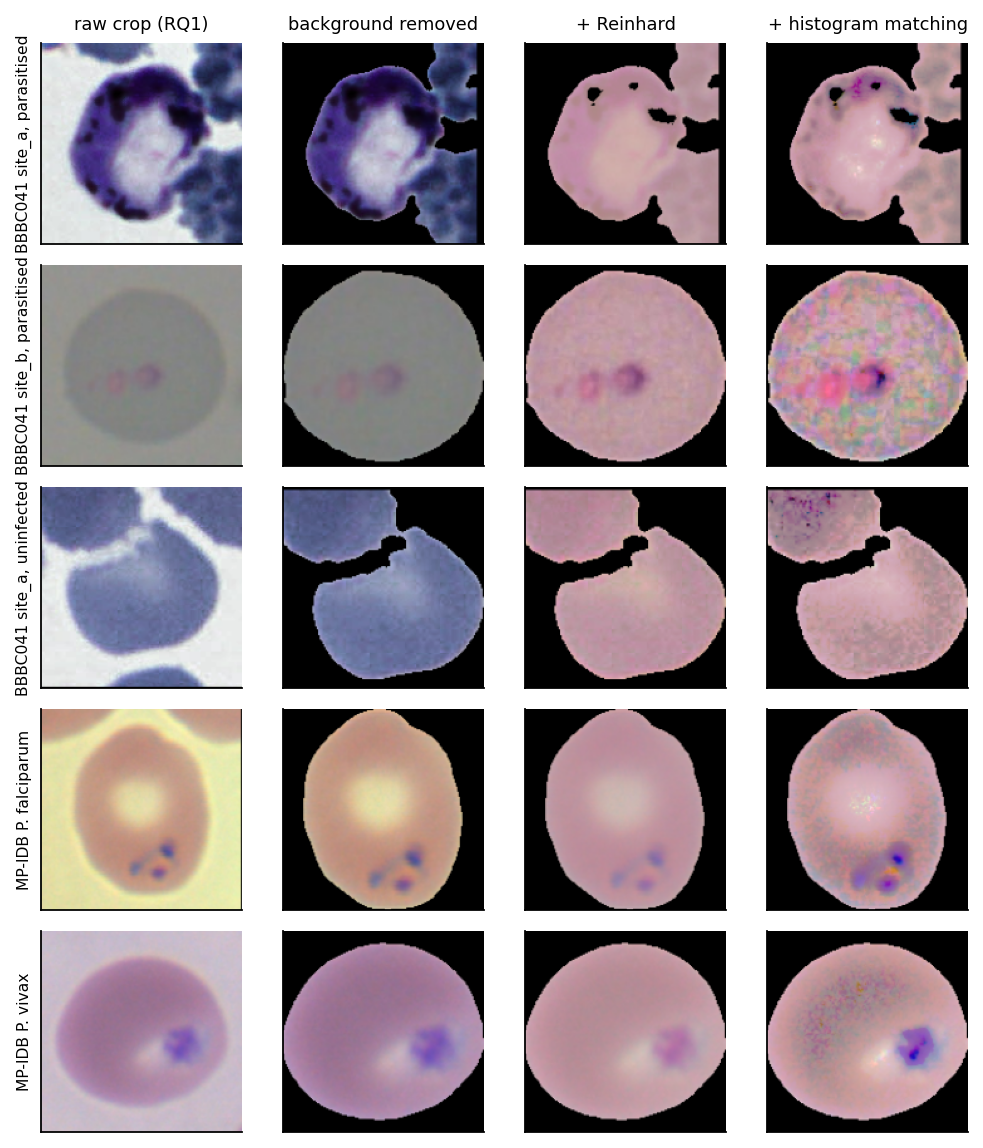
\includegraphics[width=\linewidth,height=0.66\textheight,keepaspectratio]{figures/rq2_variants.png}
\caption{The same test cells as the models see them: raw crop, background removed, and the two colour variants. Visible artefacts: Otsu keeps a touching neighbour cell (rows 1 and 3), very dark site\_a pixels are taken for background (row 1), and histogram matching amplifies the noise of grey site\_b cells (row 2). Drawn by \texttt{scripts/\allowbreak{}make\_\allowbreak{}mo\_\allowbreak{}figures.\allowbreak{}py}.}
\end{figure}

\subsection{Evaluation}

Sensitivity is the share of parasitised cells called parasitised (output above 0.5, a threshold fixed before testing), and specificity the share of uninfected cells called uninfected; drops are in percentage points (pp). They are the primary measures because BBBC041 is only 2.7 to 5.1\% parasitised, so calling every site\_a cell uninfected would score 97.3\% accuracy. AUC, the probability that a random parasitised cell scores above a random uninfected one, checks ranking without a threshold. F1 is secondary: it includes precision, the share of parasitised calls that are correct, which falls when infected cells are rare (49.2\% of NIH hold-out cells, 2.7\% of site\_a), so an F1 drop would mix model failure with prevalence (MO \S{}5.5).

\emph{Share recovered} is specific to this project: the value after a step minus the raw value, divided by the raw drop. 1 means the step closes the drop, 0 that it changes nothing, and a negative value that it widens the drop. It is computed only when the raw drop's 95\% interval lies above zero, since dividing by a drop near zero gives meaningless values. Because sensitivity also rises when a model simply calls more cells parasitised, every share is read with specificity and AUC.

Each value has a 95\% interval from a bootstrap: the test set is redrawn 2,000 times with replacement and the middle 95\% of the recomputed values kept. Whole photographs are redrawn, not cells, because cells from one photograph share its stain and focus; NIH is redrawn by patient. Training randomness is shown as the mean over three seeds with the lowest and highest seed in brackets. A finding counts as stable only if it holds in all three seeds. Models are compared on the same redrawn sets (a paired bootstrap), so luck in the draw cancels from their difference. With 24 such comparisons, about one would look real by chance at 95\%, so a Bonferroni correction widens each interval to 99.8\%. The external sets never inform training, early stopping, the colour reference or the threshold.

\section{Results, interpretation and discussion}

\subsection{RQ1: the drop and the architecture comparison}

{\scriptsize
\begin{longtable}{@{}>{\raggedright\arraybackslash}p{44.9pt}>{\raggedright\arraybackslash}p{48.9pt}>{\raggedright\arraybackslash}p{68.7pt}>{\raggedright\arraybackslash}p{68.7pt}>{\raggedright\arraybackslash}p{68.7pt}@{}}
\toprule
Test set & Model & Sensitivity & Specificity & AUC \\
\midrule
\endhead
\bottomrule
\endfoot
\bottomrule
\caption{Model comparison: mean over seeds 0 to 2 [lowest, highest seed]. NIH hold-out rows give the value (\%; AUC $\times$ 100); the other rows give the drop from that model's NIH value (pp). site\_a and site\_b are the two BBBC041 batches. Bold: smallest mean drop. Built by \texttt{scripts/\allowbreak{}make\_\allowbreak{}report\_\allowbreak{}tables.\allowbreak{}py}.}
\endlastfoot
NIH hold-out & VGG-16 & 98.0~[97.6,~98.2] & 97.0~[96.6,~97.5] & 99.6~[99.6,~99.7] \\*
 & ResNet-50 & 97.3~[97.0,~97.6] & 98.1~[97.7,~98.4] & 99.6~[99.6,~99.7] \\*
 & \mbox{MobileNetV2} & 97.2~[97.1,~97.5] & 98.0~[97.8,~98.2] & 99.6~[99.6,~99.7] \\*
site\_a & VGG-16 & \textbf{2.1~[-1.1,~6.0]} & 20.1~[13.2,~31.0] & \textbf{3.5~[2.5,~4.6]} \\*
 & ResNet-50 & 7.0~[-0.5,~17.9] & 16.5~[11.0,~19.9] & 5.6~[3.9,~7.6] \\*
 & \mbox{MobileNetV2} & 21.8~[13.4,~31.9] & \textbf{5.9~[3.2,~8.1]} & 5.7~[5.1,~6.2] \\*
site\_b & VGG-16 & \textbf{7.1~[1.6,~11.2]} & 1.3~[0.9,~1.5] & \textbf{2.2~[0.8,~3.5]} \\*
 & ResNet-50 & 30.4~[28.0,~33.9] & -0.6~[-1.3,~0.2] & 2.9~[2.2,~3.4] \\*
 & \mbox{MobileNetV2} & 59.4~[31.1,~80.2] & \textbf{-1.0~[-1.5,~-0.7]} & 8.0~[5.1,~12.3] \\*
MP-IDB \emph{P. falciparum} & VGG-16 & \textbf{33.3~[28.6,~40.9]} & - & - \\*
 & ResNet-50 & 52.9~[44.6,~59.6] & - & - \\*
 & \mbox{MobileNetV2} & 63.1~[42.4,~78.4] & - & - \\*
MP-IDB other & VGG-16 & \textbf{22.7~[18.2,~28.7]} & - & - \\*
 & ResNet-50 & 38.5~[35.6,~40.8] & - & - \\*
 & \mbox{MobileNetV2} & 61.5~[54.6,~71.4] & - & - \\*
\end{longtable}}

On the NIH hold-out the three models are close: sensitivity 97.2 to 98.0\%, specificity 97.0 to 98.1\% and AUC 0.996 (Table 1). Every external set lowers performance, but by how much depends on the model and the metric (Figure 3). VGG-16 loses the least sensitivity: 7.1 pp on site\_b against 30.4 for ResNet-50 and 59.4 for \mbox{MobileNetV2}, and 33.3 and 22.7 pp on the two MP-IDB groups against 63.1 and 61.5 for \mbox{MobileNetV2}. \mbox{MobileNetV2} never had the smallest sensitivity drop on any set in any seed, but it kept the most specificity on site\_a in every seed (drop 5.9 pp against 20.1 for VGG-16). The answer to the second half of RQ1 is therefore no: the lighter architecture does not lose less. It calls fewer external cells parasitised, which trades missed parasites for fewer false alarms. This was not expected: a small network might fit less NIH-specific detail, but the larger networks kept their sensitivity better. On site\_b the AUC drops (2.2 to 8.0 pp) are much smaller than the sensitivity drops, so much of that loss is a shift of the scores relative to the fixed threshold, with the ranking largely kept; \mbox{MobileNetV2}, with the largest AUC drop (8.0 pp), also ranks cells worse.

\begin{figure}[H]
\centering
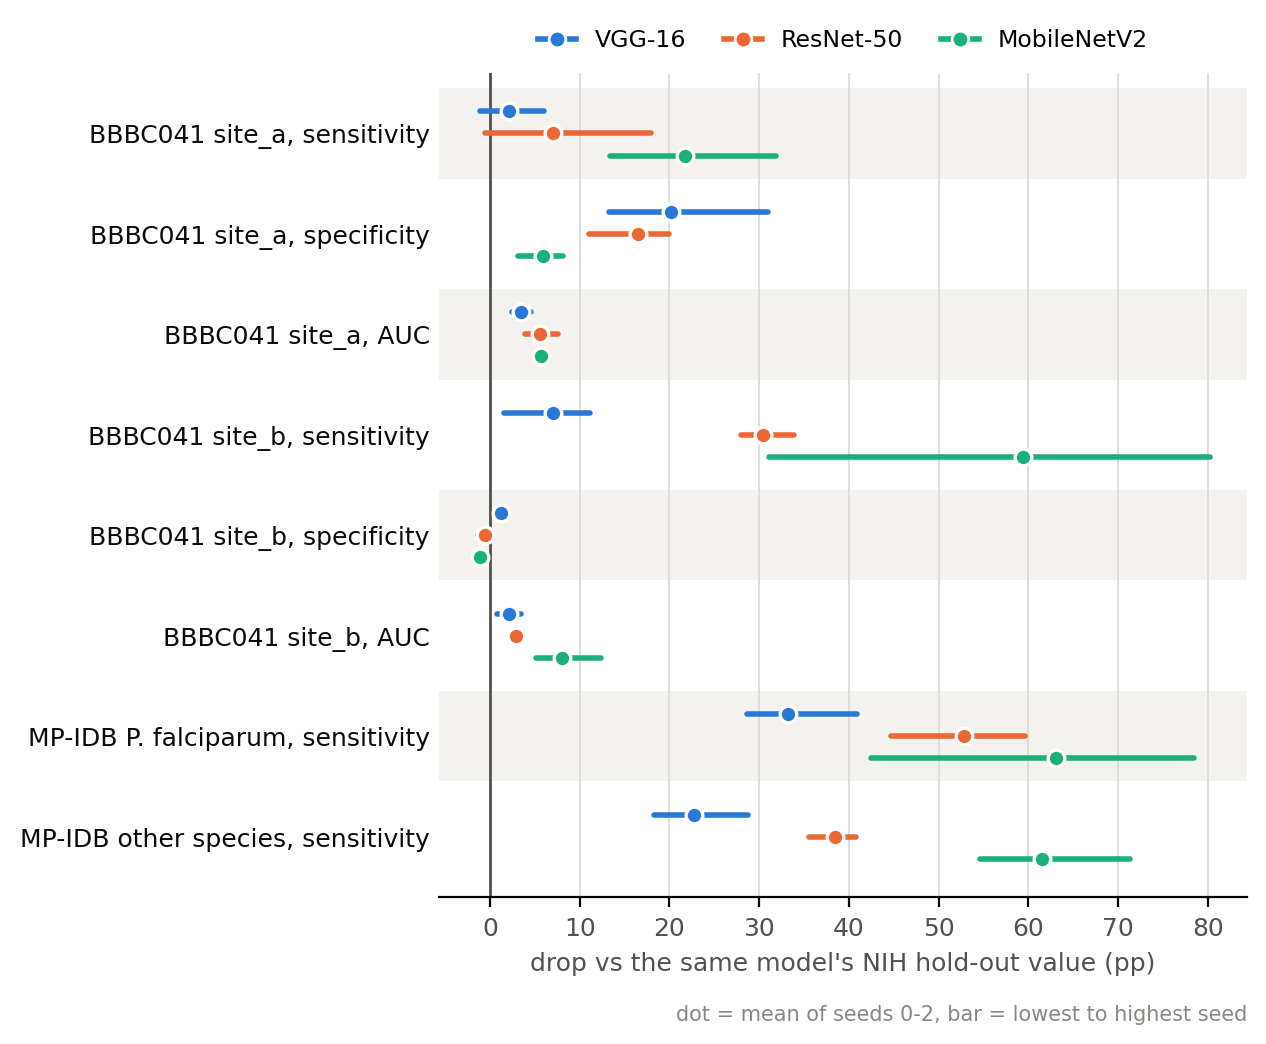
\includegraphics[width=\linewidth,height=0.66\textheight,keepaspectratio]{../../outputs/figures/report_rq1_drop.png}
\caption{Drop against each model's own NIH hold-out value, per external set and metric (dot: mean of seeds 0 to 2; bar: lowest to highest seed). Built by \texttt{scripts/\allowbreak{}make\_\allowbreak{}report\_\allowbreak{}tables.\allowbreak{}py}.}
\end{figure}

\subsection{In-sample against out-of-sample performance}

{\footnotesize
\begin{longtable}{@{}>{\raggedright\arraybackslash}p{153.4pt}>{\raggedright\arraybackslash}p{52.9pt}>{\raggedright\arraybackslash}p{52.9pt}>{\raggedright\arraybackslash}p{52.9pt}@{}}
\toprule
Data & VGG-16 & ResNet-50 & \mbox{MobileNetV2} \\
\midrule
\endhead
\bottomrule
\endfoot
\bottomrule
\caption{Sensitivity / specificity (\%) from the training data to the external sets, mean of seeds 0 to 2. Training values are measured on augmented batches at the epoch whose weights were kept. MP-IDB has no uninfected cells.}
\endlastfoot
Training (best epoch, augmented) & 96.8~/~97.7 & 96.4~/~97.7 & 96.6~/~97.9 \\*
NIH validation (best epoch) & 97.9~/~96.7 & 97.1~/~97.4 & 96.7~/~97.8 \\*
NIH hold-out & 98.0~/~97.0 & 97.3~/~98.1 & 97.2~/~98.0 \\*
BBBC041 site\_a & 95.8~/~76.9 & 90.2~/~81.5 & 75.4~/~92.1 \\*
BBBC041 site\_b & 90.9~/~95.7 & 66.9~/~98.7 & 37.8~/~99.0 \\*
MP-IDB \emph{P. falciparum} & 64.7~/~- & 44.4~/~- & 34.1~/~- \\*
MP-IDB other species & 75.2~/~- & 58.8~/~- & 35.7~/~- \\*
\end{longtable}}

Training, validation and hold-out values differ by at most 1.2 pp for every architecture (Table 2), and early stopping kept the model after 5 to 12 epochs, i.e. passes over the training data (Appendix Table A3). The models did not overfit the NIH training patients; the failure appears only on other laboratories' images, where the same models fall to 34 to 75\% sensitivity on MP-IDB. A patient-grouped hold-out set therefore says little about another laboratory.

\subsection{RQ2: matching crop format and stain colour}

Removing the background recovered part of the sensitivity drop for VGG-16 and ResNet-50, for example a share of 0.31 for ResNet-50 on MP-IDB \emph{P. falciparum} and 0.43 on site\_b (Appendix Table A1). It also lowered site\_a specificity for all three models, and mean AUC improved for no model on either BBBC041 site (Figure 4). A likely reason is two known artefacts of the masks: Otsu sometimes keeps a touching neighbour with the cell, and very dark site\_a pixels are taken for background (Figure 2), so some uninfected cells end up with dark, parasite-like fragments on black.  Reinhard transfer then lowered site\_a sensitivity by a further 34 to 43 pp, while histogram matching raised sensitivity to 85 to 100\% by calling almost every cell parasitised: site\_a specificity fell to 4.5 to 35.3\%. Its apparent recovery of 85 to 106\% of the MP-IDB drops is therefore not a gain. The answer to RQ2 is that little or none of the drop is recovered when ranking is the criterion: matching crop format and colour at test time moves scores across the threshold but does not help the models separate parasitised from uninfected cells.

\begin{figure}[H]
\centering
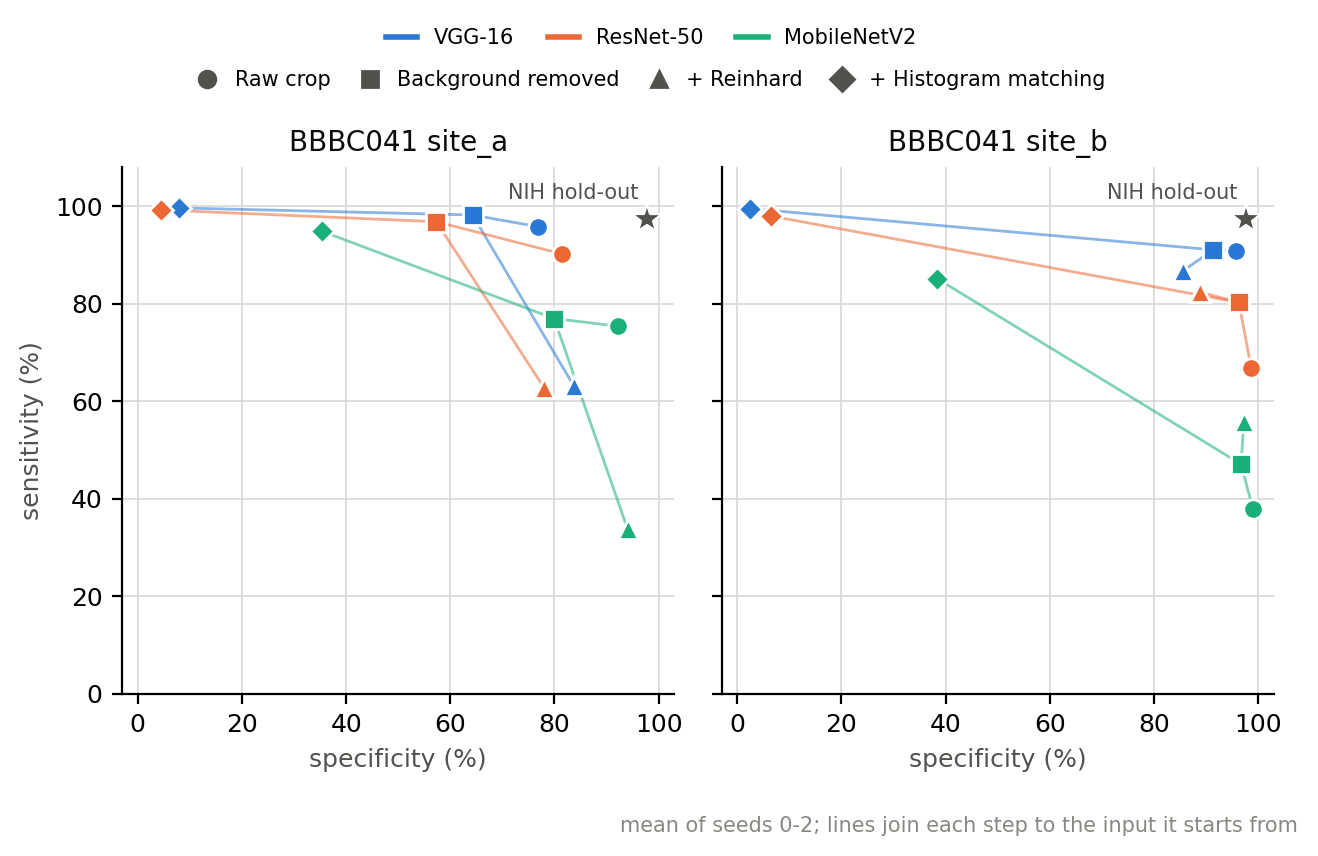
\includegraphics[width=\linewidth,height=0.66\textheight,keepaspectratio]{../../outputs/figures/report_rq2_tradeoff.png}
\caption{Sensitivity against specificity on each BBBC041 site for each test input (mean of seeds 0 to 2). The star marks the NIH hold-out. Built by \texttt{scripts/\allowbreak{}make\_\allowbreak{}report\_\allowbreak{}tables.\allowbreak{}py}.}
\end{figure}

\subsection{RQ3: species and life stages}

\emph{P. falciparum}, the training species, was detected less often than the other species in 8 of 9 runs (Appendix Table A2). The mean gap is \textminus{}10.6 pp for VGG-16 and \textminus{}14.4 pp for ResNet-50, while \mbox{MobileNetV2}'s gap changes sign between seeds. Rings account for the largest share of missed parasites on site\_b for all three models (54 to 74\%) and on site\_a for VGG-16 and ResNet-50; for \mbox{MobileNetV2} on site\_a, trophozoites (the next, larger stage) account for 53\%. Rings were also missed at a higher rate than trophozoites on site\_a in 9 of 9 runs and on site\_b in 6 of 9. Rings are small and faint, and 95\% of MP-IDB \emph{P. falciparum} parasites are rings, which plausibly explains why the training species is detected worst. Grad-CAM \citep{selvaraju2017} shows which image regions drive a prediction; applied to the first training run of each model (Appendix Figure 5), it found that the parasite received 33 to 72\% of the evidence while covering 11 to 27\% of the crop, for missed cells as much as for detected ones. This suggests the models attend to the parasite without recognising it, although \mbox{MobileNetV2} gave empty maps for over half its MP-IDB misses.

\subsection{Comparison with the literature and across seeds}

\citet{hou2026} found 96.4\% sensitivity but 18.0\% specificity on BBBC041; VGG-16 shows the same pattern in a milder form, with site\_a specificity down to 65.5\% in its worst seed while sensitivity stayed above 91\%. \citet{zhao2020} reported an AUC of 0.945 on BBBC041 for VGG-16; here VGG-16 reached 0.961 on site\_a and 0.975 on site\_b.

Seed variation is small on NIH and large on the external sets: the NIH values vary by at most 0.9 pp between seeds, while \mbox{MobileNetV2}'s site\_b sensitivity drop ranges from 31.1 to 80.2 pp. Of the 24 paired model comparisons, 18 point the same way in all three seeds, and 10 of those are also significant after Bonferroni correction in all three (\href{https://gitlab.uvt.nl/capstone/2026-fall/u927271/-/blob/main/outputs/tables/rq1_compare_seeds.csv}{\texttt{rq1\_\allowbreak{}compare\_\allowbreak{}seeds.\allowbreak{}csv}}). The RQ1 ranking holds in every seed, but single-seed numbers do not: VGG-16's site\_a specificity drop was 31.0 pp at seed 0 and 13.2 pp at seed 2. Reporting one training run, as most of the reviewed studies do, can misstate an external drop by a factor of two.

\subsection{Strengths and weaknesses}

The comparisons are fair by design: one split, identical settings, the same cells and threshold for every model and test input, paired intervals and three seeds. Every table can be rebuilt with one command, without a GPU. The weaknesses limit how far the conclusions reach. Corrections are applied only at test time, so the study cannot say whether training with colour augmentation, on masked cells or on labelled target images would remove the drop; these change the model, which RQ2 holds fixed. The fixed threshold of 0.5 mixes errors in ranking with errors in where the threshold sits, which the AUC only partly separates. The other-species group has only 140 cells, and the Grad-CAM check covers only the first training run and 100 cells per group. On BBBC041 the species and the laboratory change together, so its drop cannot be divided between them. MP-IDB has no uninfected cells, so a sensitivity gain there cannot be checked against false alarms. Colour was matched only on masked crops, so colour alone was not tested. Training settings were fixed, so the architecture ranking holds for these settings only.

\section{Conclusion, limitations and future work}

CNNs trained on NIH single cells lose much of their sensitivity on BBBC041 and MP-IDB (up to 63 pp on average) and up to 20 pp of specificity on BBBC041, yet generalise well to unseen NIH patients. The lighter \mbox{MobileNetV2} loses the most sensitivity, not the least. Matching crop format and stain colour at test time does not improve mean AUC, so these two differences, corrected this way, do not explain the drop. Rings form the largest share of misses in five of six model and site pairs, and \emph{P. falciparum} is detected less often than other species. The contribution is a controlled test-time ablation of two suspected causes, and a share-recovered measure that exposes recovery driven by the threshold.

The results rest on one source dataset, three seeds and fixed training settings. A laboratory using \mbox{MobileNetV2} at site\_b would miss most infected cells (sensitivity 38\%), so an NIH-trained model needs local validation before use (\href{https://gitlab.uvt.nl/capstone/2026-fall/u927271/-/blob/main/docs/elsa_report.md}{ELSA report}). On site\_b AUC falls far less than sensitivity, so the threshold could be re-set on a few labelled local cells, which the saved predictions can test without retraining. Test-time colour matching failed, so stain augmentation or a learned normaliser such as BeerLaNet \citep{xu2025} should be tried during training. Training data should come from several laboratories and hold more ring-stage cells.

\printbibliography[heading=ctbib,title=References]

\appendix
\setcounter{table}{0}\renewcommand{\thetable}{A\arabic{table}}

\clearpage
\section{Extended results}

{\scriptsize
\begin{longtable}{@{}>{\raggedright\arraybackslash}p{41.6pt}>{\raggedright\arraybackslash}p{38.1pt}>{\raggedright\arraybackslash}p{41.6pt}>{\raggedright\arraybackslash}p{18.4pt}>{\raggedright\arraybackslash}p{24.1pt}>{\raggedright\arraybackslash}p{31.1pt}>{\raggedright\arraybackslash}p{31.1pt}>{\raggedright\arraybackslash}p{38.1pt}@{}}
\toprule
Model & Test set & Metric & Raw & Masked & + Reinhard & + Hist. matching & Share recovered (seeds) \\
\midrule
\endhead
\bottomrule
\endfoot
\bottomrule
\caption{RQ2: drop (pp) per test input (Masked: background removed; the colour steps start from the masked crops), mean over seeds 0 to 2, and the share of the raw drop recovered by background removal (mean over the seeds in which it is defined). Seed ranges are in \texttt{outputs/\allowbreak{}tables/\allowbreak{}report\_\allowbreak{}rq2.\allowbreak{}csv}, built by \texttt{scripts/\allowbreak{}make\_\allowbreak{}report\_\allowbreak{}tables.\allowbreak{}py}.}
\endlastfoot
VGG-16 & site\_a & Sensitivity & 2.1 & -0.3 & 34.7 & -1.7 & 0.62~(2/3) \\*
 &  & Specificity & 20.1 & 32.7 & 13.3 & 89.2 & -0.76~(3/3) \\*
 &  & AUC & 3.5 & 3.9 & 14.2 & 8.4 & -0.14~(3/3) \\
 & site\_b & Sensitivity & 7.1 & 6.9 & 11.2 & -1.6 & 0.06~(2/3) \\
 &  & Specificity & 1.3 & 5.6 & 11.4 & 94.5 & n/a \\
 &  & AUC & 2.2 & 3.0 & 5.9 & 24.6 & -0.38~(3/3) \\
 & MP-IDB \emph{P. falciparum} & Sensitivity & 33.3 & 26.3 & 31.4 & -1.3 & 0.19~(3/3) \\
 & MP-IDB other & Sensitivity & 22.7 & 20.3 & 34.1 & -0.4 & 0.11~(3/3) \\
ResNet-50 & site\_a & Sensitivity & 7.0 & 0.4 & 34.5 & -2.0 & 1.07~(2/3) \\
 &  & Specificity & 16.5 & 40.7 & 20.1 & 93.5 & -1.54~(3/3) \\
 &  & AUC & 5.6 & 5.9 & 19.9 & 21.7 & -0.01~(3/3) \\
 & site\_b & Sensitivity & 30.4 & 17.0 & 14.9 & -0.7 & 0.43~(3/3) \\
 &  & Specificity & -0.6 & 1.8 & 9.2 & 91.5 & n/a \\
 &  & AUC & 2.9 & 3.3 & 6.5 & 33.9 & -0.11~(3/3) \\
 & MP-IDB \emph{P. falciparum} & Sensitivity & 52.9 & 36.0 & 42.6 & -1.6 & 0.31~(3/3) \\
 & MP-IDB other & Sensitivity & 38.5 & 22.0 & 44.7 & -2.2 & 0.43~(3/3) \\
\mbox{MobileNetV2} & site\_a & Sensitivity & 21.8 & 20.2 & 63.4 & 2.3 & 0.10~(3/3) \\
 &  & Specificity & 5.9 & 18.0 & 3.9 & 62.7 & -2.20~(3/3) \\
 &  & AUC & 5.7 & 11.6 & 14.1 & 16.4 & -1.02~(3/3) \\
 & site\_b & Sensitivity & 59.4 & 50.1 & 41.4 & 12.1 & 0.15~(3/3) \\
 &  & Specificity & -1.0 & 1.2 & 0.7 & 59.6 & n/a \\
 &  & AUC & 8.0 & 12.5 & 9.3 & 26.8 & -0.50~(3/3) \\
 & MP-IDB \emph{P. falciparum} & Sensitivity & 63.1 & 63.1 & 59.3 & 4.1 & 0.01~(3/3) \\*
 & MP-IDB other & Sensitivity & 61.5 & 60.1 & 63.4 & 9.8 & 0.03~(3/3) \\*
\end{longtable}}

{\footnotesize
\begin{longtable}{@{}>{\raggedright\arraybackslash}p{149.1pt}>{\raggedright\arraybackslash}p{31.2pt}>{\raggedright\arraybackslash}p{26.5pt}>{\raggedright\arraybackslash}p{38.1pt}>{\raggedright\arraybackslash}p{55.1pt}@{}}
\toprule
Measure & n cells & VGG-16 & ResNet-50 & \mbox{MobileNetV2} \\
\midrule
\endhead
\bottomrule
\endfoot
\bottomrule
\caption{RQ3: sensitivity by species group, and share of misses and miss rate by BBBC041 life stage, mean over seeds 0 to 2, with the number of seeds in which each finding holds. Seed ranges are in \texttt{outputs/\allowbreak{}tables/\allowbreak{}report\_\allowbreak{}rq3.\allowbreak{}csv}.}
\endlastfoot
Sensitivity, \emph{P. falciparum} (\%) & 1,297 & 64.7 & 44.4 & 34.1 \\*
Sensitivity, other species (\%) & 140 & 75.2 & 58.8 & 35.7 \\*
Gap, \emph{P. falciparum} minus other (pp) &  & -10.6 & -14.4 & -1.6 \\
... seeds where \emph{P. falciparum} detected less &  & 3/3 & 3/3 & 2/3 \\
site\_a rings, share of all misses (\%) & 353 & 43.6 & 48.7 & 19.8 \\
site\_a trophozoites, share of all misses (\%) & 1,473 & 28.2 & 41.3 & 53.0 \\
site\_a ring miss rate (\%) & 353 & 5.2 & 20.7 & 27.1 \\
site\_a trophozoite miss rate (\%) & 1,473 & 2.4 & 7.0 & 19.5 \\
... seeds where rings missed more than trophozoites &  & 3/3 & 3/3 & 3/3 \\
site\_b rings, share of all misses (\%) & 169 & 73.9 & 61.7 & 53.8 \\
site\_b trophozoites, share of all misses (\%) & 111 & 17.6 & 32.1 & 39.6 \\
site\_b ring miss rate (\%) & 169 & 11.6 & 36.7 & 60.4 \\
site\_b trophozoite miss rate (\%) & 111 & 5.1 & 28.8 & 67.6 \\*
... seeds where rings missed more than trophozoites &  & 3/3 & 3/3 & 0/3 \\*
\end{longtable}}

{\scriptsize
\begin{longtable}{@{}>{\raggedright\arraybackslash}p{50.7pt}>{\raggedright\arraybackslash}p{48.7pt}>{\raggedright\arraybackslash}p{55.3pt}>{\raggedright\arraybackslash}p{51.7pt}>{\raggedright\arraybackslash}p{30.2pt}>{\raggedright\arraybackslash}p{51.4pt}@{}}
\toprule
Model & Parameters (M) & Epochs run (seeds 0, 1, 2) & Kept epoch (seeds 0, 1, 2) & Min per epoch & Training time (min) \\
\midrule
\endhead
\bottomrule
\endfoot
\bottomrule
\caption{Model size and training effort per architecture (Colab T4 GPU).}
\endlastfoot
VGG-16 & 134.3 & 11,~15,~13 & 8,~12,~10 & 3.2 & 42~[34,~49] \\*
ResNet-50 & 23.5 & 9,~10,~8 & 6,~7,~5 & 1.8 & 16~[15,~17] \\*
\mbox{MobileNetV2} & 2.2 & 9,~10,~8 & 6,~7,~5 & 1.3 & 12~[11,~14] \\*
\end{longtable}}

{\small
\begin{longtable}{@{}>{\raggedright\arraybackslash}p{204.0pt}>{\raggedright\arraybackslash}p{132.0pt}@{}}
\toprule
Setting & Value \\
\midrule
\endhead
\bottomrule
\endfoot
\bottomrule
\caption{Training settings, identical for all nine runs (read from the training logs).}
\endlastfoot
Learning rate (Adam optimiser: step size of each weight update) & 0.0001 \\*
Batch size (images per weight update) & 32 \\*
Maximum epochs (passes over the training data) & 20 \\*
Early stopping: epochs without lower NIH validation error before training stops & 3 \\*
Weight decay (penalty on large weights) & none \\*
Input size (pixels, square) & 224 \\*
Training augmentation & horizontal and vertical flips, rotations by 90\textdegree{} \\*
Decision threshold (output above it = parasitised) & 0.5 \\*
Started from ImageNet weights, all layers trained & yes \\*
\end{longtable}}

\begin{figure}[H]
\centering
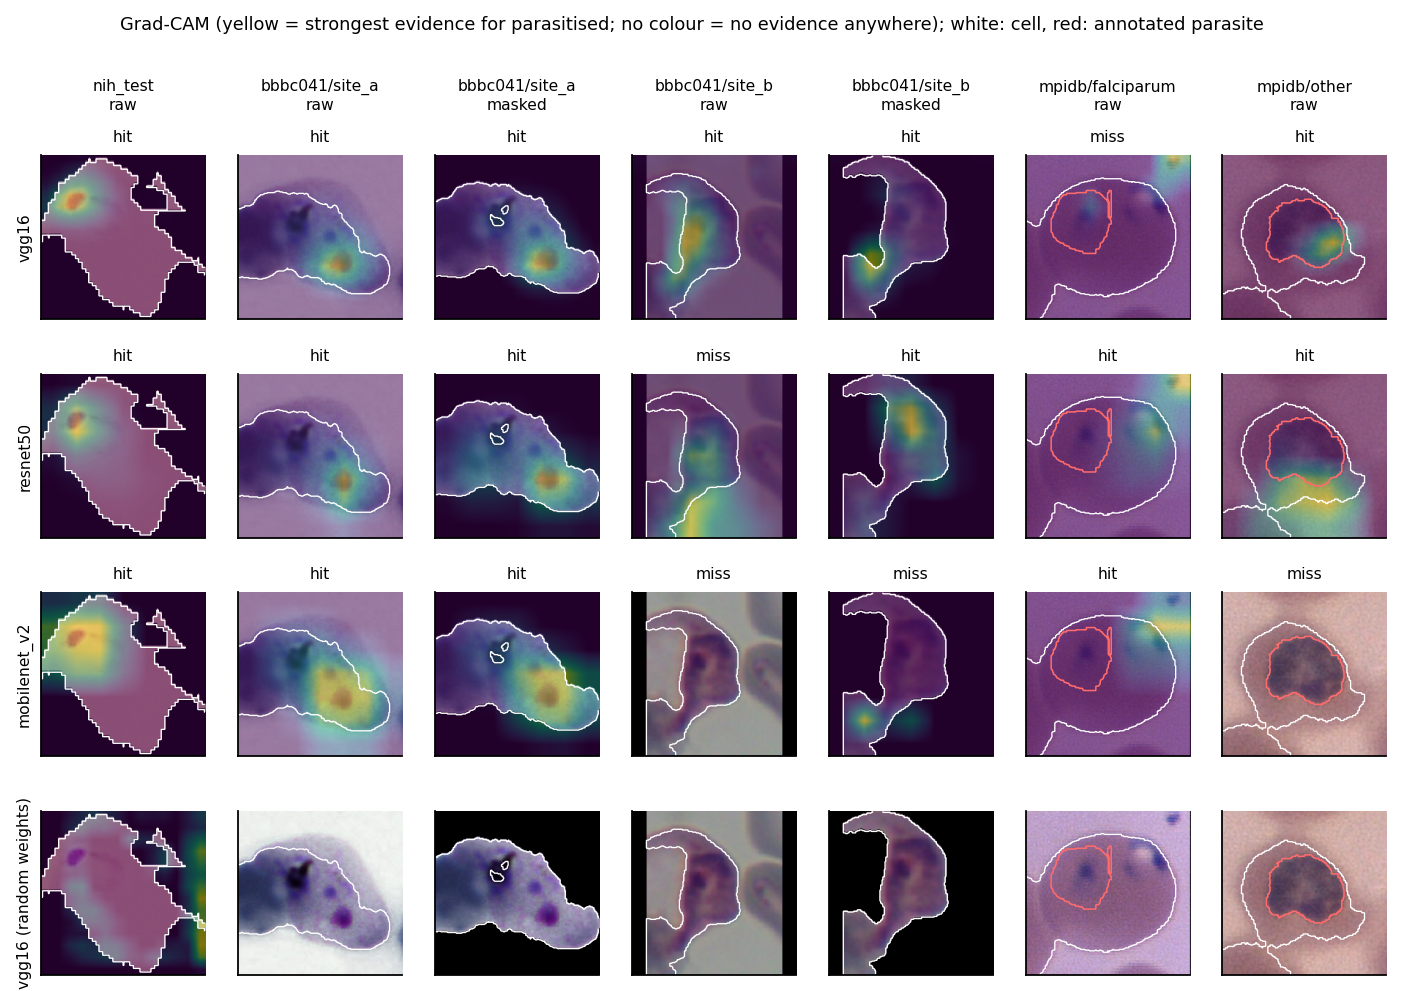
\includegraphics[width=\linewidth,height=0.66\textheight,keepaspectratio]{../../outputs/figures/gradcam_examples.png}
\caption{Grad-CAM maps of the first training run (seed 0) of each model on example cells \citep{selvaraju2017}: yellow marks the regions that most raise the predicted probability of parasitised. Drawn by \texttt{scripts/\allowbreak{}gradcam.\allowbreak{}py}.}
\end{figure}

\end{document}
